%-----------------------------------------
% Note: Use pdflatex to process this file.
%-----------------------------------------

%\documentclass{article}
\documentclass{hitec}
\usepackage{color,soul}

\usepackage{setspace}
\usepackage{graphicx}
\usepackage{moreverb}    % Defines {listing} environment.
\usepackage{amsmath, amsthm, amssymb, amsbsy, mathtools}
\usepackage{relsize}     % Make letters smaller/larger
\usepackage{alltt}
\usepackage{rotating}
\usepackage{subcaption}
\usepackage{xspace}
\usepackage[section]{placeins}   % For preventing floats from floating to end of chapter.
\usepackage{longtable}   % For splitting long vertical tables into pieces
\usepackage{index}
\usepackage{multirow}
\usepackage{booktabs}    % For table layouts
\usepackage{yhmath}      % For widehat
\usepackage{xcolor}      % Needed for listings package.
\usepackage{listings}
\usepackage[T1]{fontenc}   % so _, <, and > print correctly in text.
\usepackage[strings]{underscore}    % to use "_" in text
\usepackage[pdftex,colorlinks=true,bookmarksnumbered=true]{hyperref}   % Must be last package!


\definecolor{light-gray}{gray}{0.95}
\lstset{backgroundcolor=\color{light-gray}}
\lstset{xleftmargin=0cm}
\lstset{framexleftmargin=0.3em}
\lstset{mathescape=true}
%\lstset{basicstyle = \ttfamily\fontsize{11}{11}\selectfont} 
\lstset{basicstyle = \small}
\lstnewenvironment{code}{}{}

%---------------------------------------------------------------------------------

\definecolor{lightestgray}{gray}{0.99}
\sethlcolor{lightestgray}
\soulregister{\texttt}{1}
\newcommand\dottcmd[1]{\hl{\em#1}\endgroup}
%\newcommand\dottcmd[1]{{#1}\endgroup}
\newcommand{\vn}{\begingroup\catcode`\_=11 \catcode`\%=11 \dottcmd}
\newcommand{\Newline}{\hfil \\}
\newcommand{\sref}[1]{$\S$\ref{#1}}
\newcommand{\Sref}[1]{Sec.~\sref{#1}}
\newcommand{\Th}{$^{th}$\xspace}
\newcommand{\norm}{\text{norm}}
\newcommand{\unnorm}{\text{unnorm}}
\newcommand{\Eq}[1]{Eq.~\ref{#1}}
\newcommand{\tJ}{\widetilde J}
\newcommand{\eps}{{\mathlarger\varepsilon}}
\newcommand{\core}{\text{core}}
\newcommand{\Bf}[1]{{\bf #1}}
\newcommand{\bfN}{\Bf N}
\newcommand{\bbu}{\vn{bbu}\xspace}

%---------------------------------------------------------------------------------

\renewcommand{\textfraction}{0.1}
\renewcommand{\topfraction}{1.0}
\renewcommand{\bottomfraction}{1.0}

\settextfraction{0.9}  % Width of text
\setlength{\parindent}{0pt}
\setlength{\parskip}{1ex}
%\setlength{\textwidth}{6in}
\newcommand{\Section}[1]{\section{#1}\vspace*{-1ex}}
\newenvironment{display}
  {\vspace*{-1.5ex} \begin{alltt}}
  {\end{alltt} \vspace*{-1.0ex}}

%%% Table of Contents spacing.
\makeatletter
\renewcommand{\l@section}{\@dottedtocline{1}{1.5em}{3.3em}}
\renewcommand{\l@subsection}{\@dottedtocline{2}{3.8em}{4.2em}}
\renewcommand{\l@figure}{\@dottedtocline{1}{1.5em}{3.3em}}
\renewcommand{\l@table}{\@dottedtocline{1}{1.5em}{3.3em}}
\makeatother

%---------------------------------------------------------------------------------

\title{BBU: Beam Breakup Instability Simulation in Bmad}
\author{}
\date{David Sagan, dcs16@cornell.edu \\
William Lou, wl528@cornell.edu \\
August 12, 2023}
\begin{document}

\maketitle

%---------------------------------------------------------------------------------
\section{Overview}

\bbu is a program in \texttt{Bmad} which simulates the beam breakup instability (BBU) \cite{Bmad}. BBU occurs in recirculating accelerators due to interaction between the beam bunches and the Higher Order Modes (HOMs) in the accelerating cavities. When beam bunches go through a cavity, they are kicked by the HOM wakefields, and the kick generates orbit distortion. When the bunches return to the same cavity, their off-axis orbit through the cavity create additional wake fields. If the HOM voltage is not properly damped, this positive feedback can lead to instabilities. BBU is therefore a primary limiting factor of the maximum achievable current, the threshold current ($I_{th}$) in an Energy Recovery Linac. The point of BBU simulation is compute the $I_{th}$.

%---------------------------------------------------------------------------------
\section{Simulation detail}

The \bbu consists of two main parts: the core part written in \texttt{Fortran}, and the shell part written in \texttt{Python}. The user usually sets both BBU \texttt{Fortran} and \texttt{Python} parameters in the \texttt{Python} shell to run the simulations. The user rarely modifies the \texttt{Fortran} core. 

%---------------------------------------------------------------------------------
\subsection{Fortran core}
The core part determines the stability of a single test current by direct simulation. A train of bunches is tracked though a lattice whose cavity elements can contain HOMs (long-range wakefields). In the program, time ($t$) is measured in “turns” (abbreviated $T$). One \texttt{turn} is the time it
takes a bunch to travel from the beginning of the lattice to the end. At the start of a simulation, $t=0$, and the HOM voltages in the cavities are set to zero. Bunches are then started at
the beginning of the lattice and tracked through to the end. To minimize computation time, a single particle is used to represent each bunch.

Bunches that are initialized in the first turn period, with $0 < t <1T$, are given a random transverse offset. The offset distribution is Gaussian with default $\sigma = 10 \text{nm}$ . All bunches initialized after the first turn period will have zero transverse offset. In the tenth turn period ($9T < t < 10T$), the ``averaged maximum HOM voltage'', $V_{max}(10)$, which is the average of the strongest HOM in all the cavities within this turn, is taken as a baseline to determine whether the voltages are growing or decaying in longer turns. The reason we don't choose one of the first few turns as the baseline is because HOM voltage variation can be unstable right after initial population of the bunches. Of course, the stability of the test current should be physically independent of the choice. Also, the test current is unstable as long as one HOM voltage is growing. Therefore numerically, we only need to keep track of the strongest HOM voltage, instead of all HOM voltages.

Simulation ends when time hits the n$^{th}$ turn ($t = nT$), in which $n$ is a integer parameter set by the user ($n>10$ required). The current is declared stable or unstable depending on whether the ratio $V_{max}(n)/V_{max}(10)$ is less than or greater than 1 (or a number slightly above 1, say 1.01, to account for numerical noise), where $n$ is the number of
turns simulated (must be $>10$) set by the parameter \texttt{bbu$\_$param\%simulation$\_$turns$\_$max}. ( Strictly speaking, the \texttt{Fortran} core only outputs the ratio, and the \texttt{Python} shell determines the stability solely using this value. ) In order to shorten simulation time, ''\texttt{limit$\_$factor}'' and ``hybridization'' are implemented, and both are described below.
\bigbreak
The main input file for the \texttt{Fortran} core is ``\textcolor{red}{\texttt{bbu.init}}'', which looks like:
\begin{code}
&bbu_params 
bbu_param%lat_file_name = `erl.lat'  ! Bmad Lattice file name.
bbu_param%lat2_filename = `lat2.lat' ! For DR-scan only. 
bbu_param%simulation_turns_max = 50  ! Maximum simulation turn $n$
bbu_param%bunch_freq = 1.3e9      ! Injector bunch frequency (Hz). 
bbu_param%limit_factor = 3        ! Unstable limit to abort simulation.
bbu_param%hybridize = .true.      ! Combine non-HOM elements?
bbu_param%keep_all_lcavities = F  ! Keep all lcavities when hybridizing? 
bbu_param%current = 0.1           ! Injected test current value (A). 
bbu_param%ran_seed = 100          ! Set specific seed, 0 uses system clock. 
bbu_param%ran_gauss_sigma_cut = 3 ! Limit ran_gauss values within N$\sigma$ 
bbu_param%normalize_z_to_rf = F   ! Shift z to be in range [0, rf_wavelength]?
bbu_param%current_vary%variation_on = F !  Ramp bunch charges up and down?
!bbu_param%current_vary%...              ! Ramping parameters. 
/
\end{code}

Fortran namelist input is used. The namelist begins on the line starting with "\texttt{\&bbu_params}"
and ends with the line containing the slash ``/''. Anything outside of this is ignored. Within the
namelist, anything after an exclamation mark ``!'' is ignored, including the exclamation mark.
 
Typically \texttt{bbu.init} specifies the essential BBU parameters, but not all of them. All BBU parameters (and their default values) are defined in `\texttt{bsim/code/bbu_track_mod.f90}'. If the user includes extra parameters in \texttt{bbu.init}, the user-defined values will overwrite the default values.
The main BBU \texttt{Fortran} parameters are described below, in alphabetical order:

\begin{description}
\item[bunch_by_bunch_info_file] (string)  \Newline
If not empty, the BBU program will output orbit information of all bunches at all tracking stages. The file can be large, and is usually for debugging.
\item[bunch_freq] (float) \Newline
The injector bunch-to-bunch frequency in Hz.
%
\item[current] (float) \Newline
The injected test current in Ampere. With bunch frequency specified, this number equivalently specifies the charge of the bunches ($Q = I/f$). Note that if the bunch charge is \texttt{ramped} (See \texttt{current_vary\%variation_on}), this value is NOT the actual time-averaged current. Instead, this value determines the ``reference charge'' ($Q_{ref} = I/f$). The user must compute the actual current based on the ramping scheme. 
%
\item[current_vary\%variation_on] (boolean) \Newline
If set to True, the injector bunch charges will be ramped up and down linearly (trapezoids in time). The ramping parameters (with \texttt{current_vary} in their name) define the ramping scheme, including \texttt{t_ramp_start}, \texttt{charge_top}, \texttt{charge_bottom}, \texttt{dt_plateau}, \texttt{ramps_period}, and \texttt{dt_ramp} (See Fig. 1). 

\begin{figure}[h]
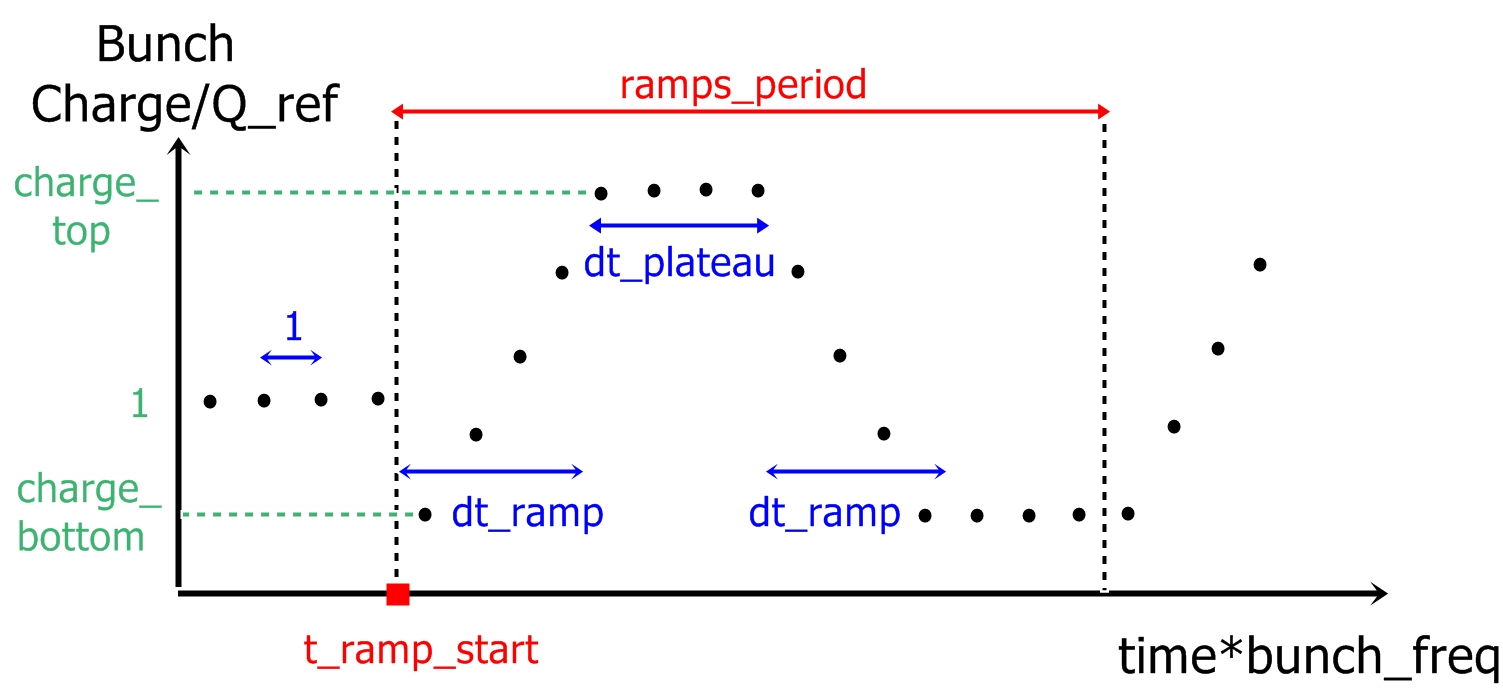
\includegraphics[scale=0.4]{BBU_code_description_ramping}
\caption{ With \texttt{current_vary\%variation_on} set to True, the bunch charge will be ramped up and down based on the ramping parameters.}
\label{setup1}
\end{figure}

Note that all the ramping parameters are dimensionless factors which have to be non-negative. That is, the two charge parameters are in unit of $Q_{ref}$ (See \texttt{bbu_param\%current}), and all the time parameters are in unit of 1/\texttt{bunch_freq}. If both \texttt{charge_top} and \texttt{charge_bottom} are set to zero, there is essentially no beam. It's acceptable to set \texttt{charge_bottom} $>$ \texttt{charge_top} to ramp down first then up. Also, it's required that (\texttt{dt_plateau} + 2$\times$\texttt{dt_ramp}) $<$ \texttt{ramps_period}.  
%
\item[drscan] (boolean)\Newline
Obsolete. The dr-scan functionality has been moved to Python shell. The associated Fortran parameters (including \texttt{elname}, \texttt{begdr}, \texttt{enddr}, and \texttt{nstep}) are also obsolete. See the section below on DR-SCAN mode for more details.

\item[ele_track_end] (string) \Newline
If specified, this is the final element in the lattice the bunches will be tracked to. The associated Fortran variable \texttt{ix_ele_track_end} is for internal use and should not be set by user.

\item[hom_order_cutoff] (integer)\Newline
If positive, ignore HOMs with order greater than this value. Default is zero. 

\item[hybridize] (boolean) \Newline
Hybridization is a process of combining all the (non-cavity) elements between any two cavities into one hybridized Taylor element. The default tracking through a hybridized element is a linear transport (see \textbf{use_taylor_for_hybrids}). This can significantly speed up calculation, with possible loss of accuracy. 
%
\item[init_particle_offset] (float) \Newline
This is the 1$\sigma$ half width, in meters, of the distribution of the initial transverse coordinates
for bunches initialized during the first turn period. The default value is 1E-10, or 10~nm.
%
\item[keep_all_cavities] (boolean) \Newline
Relevant only if \textbf{hybridize} is set to True. When hybridizing, if this is set to False, then lcavity elements that do not have HOM elements will also be hybridized. This will further speed up the simulation but can lead to inaccurate results. The recommended setting is True (see \textbf{normalize_z_to_rf}).
%
\item[keep_overlays_and_groups] (boolean) \Newline
Relevant only if \textbf{hybridize} is set to True. 
%
\item[lat_file_name] (string) \Newline
The lattice file (in Bmad standard format [2]) to be used for BBU simulation. The lattice must include at least one multipass line with at least one lcavity assigned with at least one HOM. See Bmad manual for details on lattice specification.
%
\item[limit_factor] (float) \Newline
This number has to be greater than 2.
For any intermediate turn $m$ ($10<m<n$), if the ratio $V_{max}(m)/V_{max}(10)$ is above \texttt{limit_factor}, the test current is declared unstable. If $V_{max}(m)/V_{max}(10)$ is below 1/\texttt{limit_factor}, the test current is declared stable. In either case, the program aborts so shorten simulation time.
%
\item[lat2_filename] (float) \Newline
This file is used for DR-scan only. It specifies the varied length for the `arc' element in the lattice. See DR-scan mode in the \texttt{Python} shell section below.
%
\item[normalize_z_to_rf] (boolean)\Newline
Normally, with \vn{normalize_z_to_rf} set to False (the default), the starting phase space $z$ of a
particle will reflect the time the bunch that the particle is in is launched. If RF elements are to
be hybridized, the hybrid transfer map will not work with the large $z$ values. If \vn{normalize_z_to_rf} 
is set to True, the starting $z$ values will be set to be in the range $[0, \lambda_{rf}]$ where $\lambda_{rf}$ is the
longest RF wavelength of all the cavities. In this case all the cavities must have commensurate wavelengths.
%
\item[nrep] (int) \Newline
Obsolete. 

\item[ran_seed] (integer) \Newline
Random number seed. If set to 0, the system clock will be used, and the output results will vary from run to run.
%
\item[ran_gauss_sigma_cut] (float) \Newline
Any randomized value in the lattice, such as initial orbit offset, is limited to a maximum deviation of \texttt{ran_gauss_sigma_cut} rms deviations. This is to prevent extreme values from being chosen, which can be un-physical. A typical value is between 3 to 5. The default value is -1, which means no cutoff.
%
\item[regression] (boolean) \Newline
Obsolete. The BBU regression test has been moved to be with other regression tests under the bmad-ecosystem. 

\item[simulation_turns_max] (integer) \Newline
The maximum number of simulation turn the program runs up to when no particle loss is detected. Must be greater than 10. A large number slows down the computation, but increases accuracy. A typical choice is between 50 to 300. 
%
\item[stable_orbit_anal] (boolean)\Newline
If True, write stable_orbit.out and hom_voltage.out (for debugging).
%
\item[use_taylor_for_hybrids] (boolean) \Newline
Relevant only if \textbf{hybridize} is set to True. Use taylor map for hybrids when True, otherwise the tracking method is linear. Default is False.
%
\item[write_digested_hybrid_lat] (boolean) \Newline
For debugging purposes.
\item[write_voltage_vs_time_dat] (boolean) \Newline
For debugging purposes. If true, write a (large) output file which contains the maximum_HOM_voltage data at every tracking step. The user can plot the data to visually check the stability of the test current. This is probably the most reliable way to check whether the test current is stable, because the stability behavior can be unclear if total simulation time is too short, or if the no clear divergence or steady-state occurs to the program.

\end{description}

%---------------------------------------------------------------------------------
\subsection{Python Shell/Wrapper}
Since the \texttt{Fortran} core program only determines the stability of ONE test current, multiple runs of the core (with different test currents) are required to pin down the $I_{th}$. This can be done with the developed Python shell which interacts calls the core program. Besides finding the $I_{th}$ of a specific design, the shell can also generate statistics of $I_{th}$ by introducing small variations to either the lattice or the HOM assignments. Each type of variation is considered as a ``simulation mode'' (See Section below). 

The main file for the \texttt{Python} shell is \textcolor{red}{\texttt{test_run.py}}, in which the user specifies all the BBU (\texttt{Fortran}) parameters and additional \texttt{Python} parameters. Other associated \texttt{Python} codes are under the \texttt{\$DIST_BASE_DIR/bsim/bbu/python/} directory. The user should make sure this directory is included in the environment variable \texttt{PYTHONPATH}.

The most important \texttt{Python} parameters which are common to all the simulation modes are:

\begin{description}
\item[exec_path] \Newline
The exact path of the compiled BBU \texttt{Fortran} program. Typically this is under the \texttt{.../production/bin/} directory. 
%
\item[threshold_start_curr] \Newline
Initial guess of the test current. An educational guess based on the lattice design and HOM assignments can reduce the total simulation time. 
%
\item[final_rel_tol] \Newline
\texttt{Python} shell iteratively calls the  \texttt{Fortran} core to pin down the $I_{th}$. This value determines accuracy of the $I_{th}$ found.
\end{description}

The existing Python shell has limited functionalities, so users are encouraged to write their own wrapper with external programs for independent BBU studies. For instance, multiple BBU runs with different test currents can be run in parallel. Also, by importing data from the \texttt{write_voltage_vs_time_dat} output, one can write their own function to determine the BBU stability.  
%---------------------------------------------------------------------------------
\section{Simulation Modes}
The user can run different simulation modes by adjust the arguments passed to  \texttt{test_run.py}. The details of each mode and their additional \texttt{Python} parameters are described below. Note that regardless of the mode, original lattice MUST have a valid initial HOM assignment. 

%---------------------------------------------------------------------------------
\subsection{DR-SCAN mode}
\textcolor{blue}{Number of argument: 0}
\bigbreak
Run this command under \texttt{ \$DIST_BASE_DIR/bsim/bbu/examples} :
\\
\textcolor{blue}{\texttt{python   \$DIST_BASE_DIR/bsim/bbu/test_run.py}} 
\bigbreak
Obtain ($I_{th}$ v.s $t_r/t_b$) for a lattice with a varying arc length. ($t_r$ is the recirculation time, and $t_b$ is 1/\texttt{bunch_freq}). The lattice must have a unique element named ``\texttt{arc}'' of which the length ($t_r \times$ speed of light) is varied.
This mode produced the plot for Fig.3 in \cite{GeorgBBU} and Fig.14 in \cite{WlouBBU}, for which one dipole HOM is assigned to one cavity in a lattice with one recirculation pass (the simplest BBU model). This mode is commonly used to check if the simulation agrees with the theory, as shown in the two papers.
\bigbreak
\texttt{Python} Parameters:

1) \texttt{start_dr_arctime}: $t_r$ (in seconds) of the first data point.

2) \texttt{end_dr_arctime}: $t_r$ (in seconds) of the final data point.

3) \texttt{n_data_pts_DR}: number of data points. Must be a positive integer. If equal to 1, \texttt{end_dr_arctime} is ignored. Decrease this for fast result with fewer evaluation points.

4) \texttt{plot_drscan}: If True, the \texttt{Python} program will produce a plot of ($I_{th}$ v.s $t_r/t_b$). The user must exit the plot to obtain the data in an output file. This must be set to False for grid job submission.  

\bigbreak
Output file: \texttt{thresh_v_trotb.txt}

%---------------------------------------------------------------------------------
\subsection{THRESHOLD mode}      
\textcolor{blue}{Number of argument: 3}
\bigbreak
Command: \textcolor{blue}{\texttt{python \$DIST_BASE_DIR/bsim/bbu/test_run.py  \text{} N \text{} fn \text{} output_dir }}
\bigbreak
Compute the $I_{th}$ for \texttt{N} times for a fixed lattice, each time with a (random) set of HOM assignment. It is recommended to set \texttt{N} = 1 and use parallel computation. \texttt{fn} is the string used to distinguish between the simulation runs, and can be set to the job number (\texttt{\$JOB_ID}) during grid submission.

\bigbreak
\texttt{Python} Parameters:

1) \texttt{random_homs}: If True, the original HOM assignment to the lattice will be over-written by a HOM assignment file  randomly chosen from ``\texttt{hom_dir}''.
The simulation result ($I_{th}$ found) will be generally different over multiple runs. 
If False, the program will be seeking a file in the working directory (the directory where the user calls the \texttt{Python} program) named ``\texttt{assignHOMs.bmad}'' in attempt to over-write the original assignment. If ``\texttt{assignHOMs.bmad}'' is not present, the original assignment is intact, but the user will have to manually record the assignment. 

2) \texttt{hom_dir}:
The exact path of the HOM assignment files to be randomly assigned. Each file must be named ``\texttt{cavity_I.dat}'', in which \texttt{I} is presumably a positive integer.

\bigbreak
Output file:  \texttt{bbu_threshold_fn.txt}, which includes $I_{th}$ (if found) and, if overwritten, the HOMs assigned to the cavities.

%---------------------------------------------------------------------------------
\subsection{PHASE_SCAN mode}
\textcolor{blue}{Number of argument: 1}
\bigbreak
Command:  \textcolor{blue}{\texttt{python \$DIST_BASE_DIR/bsim/bbu/test_run.py  PHASE}}

Obtain ($I_{th}$ v.s. $\phi$) for a lattice with a varying horizontal phase-advance $\phi$. The phase advance is changed via a zero-length first-order \texttt{Taylor} element (See Bmad manual for detail.) named ``taylorW'', which is equivalent to a 2x2 transfer matrix $M(\phi)$ in the horizontal phase space:

\[
M(\phi) =
\begin{pmatrix}
   (\cos\phi+\alpha_{x}\sin\phi) & \beta_{x}\sin\phi \\ 
  \gamma_{x}\sin\phi &  (\cos\phi-\alpha_{x}\sin\phi)
\end{pmatrix}
\]


The user must include ``taylorW'' in the lattice in order to run the phase_scan mode. To preserve the beam optics of the original lattice, the Twiss parameters ($\beta_x, \alpha_x$) at where taylorW locates must be extracted from the lattice, and set in \texttt{.../bsim/bbu/python/bbu/phase_scan.py}. Due to periodicity, $\phi$ is only needs to be scanned from 0 to 2$\pi$.
       
\bigbreak
\texttt{Python} Parameters:

1) \texttt{start_phase}: $\phi$ of the first data point for \texttt{n_data_pts_PHASE} $>=2$. Default is zero.

2) \texttt{end_phase}: $\phi$ of the final data point for \texttt{n_data_pts_PHASE} $>=2$. Default is 2$\pi$.

3) \texttt{n_data_pts_PHASE}: number of data points. Must be a positive integer. If equal to 1, only the input \texttt{PHASE} is scanned. If $>=2$, the input \texttt{PHASE} is ignored.

4) \texttt{ONE_phase}: will store the input value of \texttt{PHASE}.  No need to modify.

5) \texttt{plot_phase_scan}: If True, the \texttt{Python} program will produce a plot of ($I_{th}$ v.s $\phi$). The user must exit the plot to obtain the data. This must be set to False for grid jobs.  

\bigbreak
Output file: \texttt{thresh_v_phase_PHASE.txt}

%---------------------------------------------------------------------------------
\subsection{PHASE_SCAN_XY mode}
\textcolor{blue}{Number of argument: 2}
\bigbreak
Command:  \textcolor{blue}{\texttt{python3 .../bsim/bbu/test_run.py  PHASE_X  PHASE_Y }}

\bigbreak
(1) Decoupled case: Obtain ($I_{th}$ v.s. ($\phi_x$, $\phi_y$)) for a lattice with varying phase-advances in both X and Y (optics decoupled).

(2) Coupled case: Obtain ($I_{th}$ v.s. ($\phi_1$, $\phi_2$)) for a lattice with two varying phases with X-Y coupling.

\bigbreak
Similar to the PHASE_SCAN mode, talylorW is introduced, but this time as a 4x4 matrix:

  

\[
T_{decoupled}(\phi_{x},\phi_{y}) =
\begin{pmatrix}
   M_{x\leftarrow x} (\phi_{x}) & \boldsymbol{0}    \\
  \boldsymbol{0}  &  M_{y\leftarrow y} (\phi_{y}) 
\end{pmatrix}
\]
\[
T_{coupled}(\phi_{1},\phi_{2}) =
\begin{pmatrix}
  \boldsymbol{0}   & M_{x\leftarrow y} (\phi_{1})   \\
   M_{y\leftarrow x} (\phi_{2})   & \boldsymbol{0}
\end{pmatrix}
\]

, in which $M(\phi)$ is a the 2x2 transfer matrix in terms of the Twiss parameters:
\[
M_{1 \leftarrow 0}(\phi) =
\begin{pmatrix}
  \sqrt{\frac{\beta_{1}}{\beta_{0}}} (\cos\phi+\alpha_{0}\sin\phi) & \sqrt{\beta_{1} \beta_{0}}\sin\phi \\ 
  \frac{1}{\sqrt{\beta_{1}\beta_{0}}}[(\alpha_{0}-\alpha_{1})\cos\phi-(1+\alpha_{0}\alpha_{1})\sin\phi] & \sqrt{\frac{\beta_{1}}{\beta_{0}}} (\cos\phi-\alpha_{1}\sin\phi) 
\end{pmatrix}
\]

For the decoupled case, the two phases are the conventional transverse phase advances. If \texttt{PHASE_Y = 0}, this is equivalent to the phase scan mode. For the coupled case, the input argument \texttt{PHASE_X} is used as $\phi_1$, and \texttt{PHASE_Y} is used as $\phi_2$.
To use either the decoupled or coupled case, the user must extract the Twiss parameters ($\beta_x, \alpha_x$, $\beta_y$, $\alpha_y$) at where taylorW locates, and set them in \texttt{.../bsim/bbu/python/bbu/phase_scan.py}.

For a complete scan of over the two phases (both from 0 to 2$\pi$), parallel computation is recommended. 

\bigbreak
\texttt{Python} Parameters:

1) \texttt{phase_x}: will store the input value of \texttt{PHASE_X}. No need to modify.

2) \texttt{phase_y}: will store the input value of \texttt{PHASE_Y}. No need to modify.

3) \texttt{xy_coupled}: (important) 0 for the decoupled case; 1 for the coupled case. 


\bigbreak     
Output file: \texttt{thresh_v_phase_PHASE_X_PHASE_Y.txt} 

%---------------------------------------------------------------------------------
\section{Important files}
\subsection{BBU Fortran codes}
The files with core computation.

1)\texttt{\$DIST_BASE_DIR/bsim/bbu/bbu_program.f90}: Main BBU program.

2)\texttt{\$DIST_BASE_DIR/bsim/code/bbu_track_mod.f90}: BBU tracking and computation modules.

%---------------------------------------------------------------------------------
\subsection{ Python main user interface }
The Python wrapper which interacts with the Fortran core.

1) \texttt{\$DIST_BASE_DIR/bsim/bbu/test_run.py}: 
The TOP interface file which defines all BBU \texttt{Fortran} and \texttt{Python} parameters ( to be modified by the user ).
When run, a temporary directory is created, which contains \texttt{bbu.init} and associated filed to run the \texttt{Fortran} core for multiple times. The directory is cleaned up at the end of the Python program. The user can deliberately terminate the \texttt{Python} program to investigate the temporary files (for debugging).


%---------------------------------------------------------------------------------
\subsection{Python package}
These files are for intermediate  organization and communication between \texttt{test_run.py} and the \texttt{Fortran} core.

(Location: \texttt{.../bsim/bbu/python/bbu/})(Make sure \texttt{.../bsim/bbu/pyhton/} is included in the environment variable \texttt{\$PYTHONPATH}.)

1) \texttt{bbu_main.py}: Parse results from the \texttt{Fortran} code. Calls other \texttt{Python} codes.

2) \texttt{find_threshold.py}: Calculates new test current (or reference charge). Prepare temporary files to run the \texttt{Fortran} core.

3) \texttt{drscan.py}: Prepares drscan files (\texttt{lat2.lat}) and plot.

4) \texttt{phase_scan.py}: Prepares phase\_scan (or phase\_xy\_scan) files (\texttt{lat2.lat}) and plot.

%---------------------------------------------------------------------------------
\subsection{Others}
Potentially useful files. 

1) \texttt{collect_thresholds.py}: this \texttt{Python} program summarizes the calculated threshold currents stored in the local "bbu\_thresholds\_*" output files. The output file is bbu\_combined\_thresholds.txt.

2) \texttt{assignHOMs.bmad}: If this file exists in the directory which the user calls \texttt{test_run.py}  (not necessarily the directory where \texttt{test_run.py} locates), the HOM assignment from the original lattice will be over-written, unless the user has specified \texttt{py_par[`random_homs']} to be True.


%---------------------------------------------------------------------------------
\begin{thebibliography}{99}

\bibitem{Bmad}
David Sagan. {\em The Bmad Reference Manual},\\
{\em https://www.classe.cornell.edu/bmad/manual.html}

\bibitem{GeorgBBU} 
G.H.~Hoffstaetter, I.V.~Bazarov, \emph{Beam-Breakup Instability Theory for Energy Recovery Linacs},
Phys.~Rev.~ST-AB {\bf 7}, 054401 (2004).

\bibitem{WlouBBU}
W.~Lou, G.H.~Hoffstaetter, \emph{BBeam breakup current limit in multiturn energy recovery linear accelerators},
Phys.~Rev.~ST-AB {\bf 22}, 112801 (2019).

\end{thebibliography}

\end{document}

